\documentclass[]{article}
\usepackage{lmodern}
\usepackage{amssymb,amsmath}
\usepackage{ifxetex,ifluatex}
\usepackage{fixltx2e} % provides \textsubscript
\ifnum 0\ifxetex 1\fi\ifluatex 1\fi=0 % if pdftex
  \usepackage[T1]{fontenc}
  \usepackage[utf8]{inputenc}
\else % if luatex or xelatex
  \ifxetex
    \usepackage{mathspec}
  \else
    \usepackage{fontspec}
  \fi
  \defaultfontfeatures{Ligatures=TeX,Scale=MatchLowercase}
\fi
% use upquote if available, for straight quotes in verbatim environments
\IfFileExists{upquote.sty}{\usepackage{upquote}}{}
% use microtype if available
\IfFileExists{microtype.sty}{%
\usepackage{microtype}
\UseMicrotypeSet[protrusion]{basicmath} % disable protrusion for tt fonts
}{}
\usepackage[margin=1in]{geometry}
\usepackage{hyperref}
\hypersetup{unicode=true,
            pdftitle={Einfache Korpusanalysen: Ein Schnelleinstieg},
            pdfauthor={Stefan Hartmann},
            pdfborder={0 0 0},
            breaklinks=true}
\urlstyle{same}  % don't use monospace font for urls
\usepackage{longtable,booktabs}
\usepackage{graphicx,grffile}
\makeatletter
\def\maxwidth{\ifdim\Gin@nat@width>\linewidth\linewidth\else\Gin@nat@width\fi}
\def\maxheight{\ifdim\Gin@nat@height>\textheight\textheight\else\Gin@nat@height\fi}
\makeatother
% Scale images if necessary, so that they will not overflow the page
% margins by default, and it is still possible to overwrite the defaults
% using explicit options in \includegraphics[width, height, ...]{}
\setkeys{Gin}{width=\maxwidth,height=\maxheight,keepaspectratio}
\IfFileExists{parskip.sty}{%
\usepackage{parskip}
}{% else
\setlength{\parindent}{0pt}
\setlength{\parskip}{6pt plus 2pt minus 1pt}
}
\setlength{\emergencystretch}{3em}  % prevent overfull lines
\providecommand{\tightlist}{%
  \setlength{\itemsep}{0pt}\setlength{\parskip}{0pt}}
\setcounter{secnumdepth}{5}
% Redefines (sub)paragraphs to behave more like sections
\ifx\paragraph\undefined\else
\let\oldparagraph\paragraph
\renewcommand{\paragraph}[1]{\oldparagraph{#1}\mbox{}}
\fi
\ifx\subparagraph\undefined\else
\let\oldsubparagraph\subparagraph
\renewcommand{\subparagraph}[1]{\oldsubparagraph{#1}\mbox{}}
\fi

%%% Use protect on footnotes to avoid problems with footnotes in titles
\let\rmarkdownfootnote\footnote%
\def\footnote{\protect\rmarkdownfootnote}

%%% Change title format to be more compact
\usepackage{titling}

% Create subtitle command for use in maketitle
\providecommand{\subtitle}[1]{
  \posttitle{
    \begin{center}\large#1\end{center}
    }
}

\setlength{\droptitle}{-2em}

  \title{Einfache Korpusanalysen: Ein Schnelleinstieg}
    \pretitle{\vspace{\droptitle}\centering\huge}
  \posttitle{\par}
    \author{Stefan Hartmann}
    \preauthor{\centering\large\emph}
  \postauthor{\par}
      \predate{\centering\large\emph}
  \postdate{\par}
    \date{2019-06-10}

\renewcommand{\figurename}{Fig.}
\renewcommand{\contentsname}{Inhalt}

\begin{document}
\maketitle

{
\setcounter{tocdepth}{2}
\tableofcontents
}
\section{Einstieg}\label{einstieg}

Ziel dieses Tutorials ist es, Anfänger*innen einen möglichst
niedrigschwelligen Einstieg in einfache Korpusanalysen zu ermöglichen.
Es ist insbesondere für Studierende gedacht, die z.B. für eine
Seminararbeit eine Korpusrecherche durchführen möchten, aber bislang
noch keine praktische Erfahrung mit korpuslinguistischen Methoden
sammeln konnten. Das Tutorial bietet anhand eines konkreten Beispiels
eine Schritt-für-Schritt-Anleitung, wie man von der Fragestellung zur
Datengewinnung hin zur Analyse der Daten gelangen kann.

Um wirklich einen Schnelleinstieg bieten zu können, muss ich
notwendigerweise vieles vereinfachen. Für Ihre konkrete Korpusstudie
werden Sie daher wahrscheinlich nicht umhinkommen, sich an der einen
oder anderen Stelle tiefer einzulesen. Dafür verweise ich im Text immer
wieder auf weiterführende Ressourcen. Teilweise finden sich auch in
diesem Tutorial vertiefende Passagen, die Sie aufklappen können:

 ‣ \textbf{klick mich}

Hallo, ich bin eine vertiefende Passage.

Sonst gibt es hier nichts zu sehen. Sie können mich gern wieder
schließen. Danke.

\section{Von der Fragestellung zur
Konkordanz}\label{von-der-fragestellung-zur-konkordanz}

Die meisten empirischen Studien lassen sich auf folgende Schritte
herunterbrechen:

\begin{itemize}
\tightlist
\item
  Eine Fragestellung formulieren
\item
  Daten erheben
\item
  Daten auswerten.
\end{itemize}

\subsection{Eine Fragestellung
formulieren}\label{eine-fragestellung-formulieren}

Der erste Schritt ist wahrscheinlich der wichtigste. Nur wenn Sie eine
gute Forschungsfrage haben, können Sie eine aussagekräftige empirische
Analyse durchführen. Aus der Forschungsfrage ergibt sich die Methode:
Für manche Fragestellungen bietet sich z.B. eine Fragebogenstudie an,
für eine eine psycho- oder neurolinguistische Herangehensweise, für
wieder andere eine Korpusrecherche.

Das heißt auch: Wenn Sie eine Korpusanalyse durchführen möchten,
brauchen Sie eine Fragestellung, die korpuslinguistisch
operationalisierbar ist. Beispielsweise lässt sich eine Frage wie
``Welche Gehirnareale werden beim Hören von Bewegungsverben aktiviert?''
natürlich nicht mit Hilfe von Korpusdaten beantworten.

Für unsere Beispielanalyse werfen wir einen Blick auf die prädikative
Verwendung der Partizipien \emph{programmiert} und
\emph{vorprogrammiert}. Letzteres ist manchen Sprachpflegern ein Dorn im
Auge: So bezeichnet es Batian Sick als

\begin{quote}
``umgangssprachliches Blähwort, über das schon Heerscharen von
Sprachpflegern hergefallen sind -- vergebens, denn es wird immer munter
weiter vorprogrammiert. Dabei wissen nicht nur Programmierer: Man
programmiert immer im Voraus, die Vorsilbe vor- ist daher pleonastisch,
zu Deutsch: doppelt gemoppelt.'' \hfill ---
\url{https://bastiansick.de/kolumnen/abc/vorprogrammiertprogrammiert/}
\end{quote}

Was Sprachpfleger wie Sick jedoch oft verkennen, ist, dass Sprache nicht
immer ``logisch'' ist. Vielmehr suchen sich Wörter oft eigene Nischen.
Beispielsweise ist mein Bürostuhl kein \emph{Rollstuhl}, obwohl er
Rollen hat - denn das Wort \emph{Rollstuhl} hat eine eigene Bedeutung
angenommen, die sich nicht kompositional aus seinen Einzelteilen ergibt.
Im Falle von \emph{vorprogrammiert} hingegen passt zwar die Paraphrase
`im Voraus programmiert'. Aber trotzdem wäre denkbar, dass das Wort eine
Spezialisierung erfahren hat: Wird \emph{programmiert} möglicherweise
eher dann verwendet, wenn ein Programmierungsvorgang im wörtlichen Sinn
gemeint ist, und \emph{vorprogrammiert} eher dann, wenn ein z.B. ein
Skandal oder eine Katastrophe ``vorprogrammiert'' sind? Das ist die
Fragestellung, der wir im Folgenden nachgehen möchten.

 ‣ \textbf{Fragestellungen und Hypothesen}

Die Unterscheidung von \textbf{Fragestellung} und \textbf{Hypothese}
bereitet Anfänger*innen oft Schwierigkeiten. Beide hängen eng zusammen.
In unserem Beispiel könnte man die Frage in eine Hypothese
umformulieren: ``vorprogrammiert wird eher in metaphorischem und
programmiert eher im wörtlichen Sinn verwendet.''

Hypothesen ergeben sich in der Regel aus konkreten Fragestellungen.
Beispielsweise könnte in einer soziologischen oder
politikwissenschaftlichen Studie die Fragestellung lauten: Welchen
Einfluss hat das Alter auf das Wahlverhalten in Deutschland? Da man zu
diesem Themengebiet aus der bisherigen Forschung und aus der
Alltagserfahrung das eine oder andere schon weiß, kann man begründete
Annahmen darüber treffen, wie die Antwort auf diese Frage aussieht. So
könnte man davon ausgehen, dass z.B. ältere Menschen eher etablierte und
vielleicht auch eher konservative Parteien wählen und dass außerdem bei
Älteren eine höhere Wahlbeteiligung vorliegt. Diese Annahmen nennt man
Hypothesen. Sie werden auf Grundlage der Daten, die man erhebt,
überprüft.

Nicht immer ist es möglich oder notwendig, konkrete Hypothesen zu
formulieren. Gerade bei Phänomenen, über die noch sehr wenig bekannt
ist, bietet es sich manchmal an, \textbf{explorativ}, also
``erkundend'', zu arbeiten. Auch dann gehe ich mit einer Fragestellung
an meine Daten heran, ohne jedoch im Voraus eine Erwartung zu haben, wie
die Antwort auf meine Frage aussehen wird.

\subsection{Daten erheben}\label{daten-erheben}

\subsubsection{Suchsyntax}\label{suchsyntax}

Für die Datenerhebung verwenden wir das DWDS-Kernkorpus des 20.
Jahrhunderts, das über dwds.de zugänglich ist. Wir suchen auf der
Wortebene mit Hilfe von regulären Ausdrücken nach den Formen
\emph{programmiert} und \emph{vorprogrammiert}. Dafür benutzen wir den
Suchstring
\texttt{@programmiert\ \textbar{}\textbar{}\ @vorprogrammiert}. Das
@-Zeichen bedeutet, dass wir genau diese Strings suchen und keine
anderen Wortformen wie \emph{programmierte}, \emph{programmiertes} etc.
Da uns nur die prädikative Verwendung interessiert, brauchen wir die
flektierten Wortformen nicht. Der horizontale Strich \textbar{} ist der
ODER-Operator; dass man ihn hier doppelt setzen muss, ist eine
Besonderheit der DWDS-Suchsyntax.

‣ \textbf{Alternative Suchabfrage mit regulären Ausdrücken} Alternativ
können wir das gleiche Ergebnis auch durch Verwendug regulärer Ausdrücke
erzielen: \texttt{\$w=/(vor)?programmiert/g}. Ich ermutige alle, die
sich mit Korpuslinguistik beschäftigen wollen, sehr, sich mit regulären
Ausdrücken vertraut zu machen. Allerdings unterstützt die
DWDS-Suchsyntax reguläre Ausdrücke derzeit nur in sehr beschränktem
Maße. (Deutlich besser ist in dieser Hinsicht das alternative
Abfrageportal Dstar, das jedoch für Anfänger*innen nur bedingt geeignet
ist.)

 ‣ \textbf{Zur Suche im DWDS und anderswo} - Die Hilfe zur Suche im DWDS
findet sich hier.

\begin{itemize}
\item
  Einen Einstieg in reguläre Ausdrücke bietet z.B.
  regular-expressions.info.
\item
  In den Begleitmaterialien zu meiner ``Deutschen Sprachgeschichte''
  finden sich ebenfalls einige Tutorials zur Suche in einschlägigen
  Korpora.
\item
  Sehr empfehlenswert und erfreulich ausführlich ist außerdem die
  Korpuslinguistik-Seite von Noah Bubenhofer. 
\end{itemize}

\subsubsection{Export}\label{export}

Die Suche liefert uns 88 Treffer, die nun im Browser in ihrem jeweiligen
Kontext dargestellt werden. Diese Daten wollen wir nun exportieren, und
zwar im ``Key Word in Context'' (KWIC)-Format. Damit ist gemeint, dass
der Suchtreffer zusammen mit seinem unmittelbaren Kontext dargestellt
wird. Erfreulicherweise bietet das DWDS eine sehr gute Exportfunktion,
die es erlaubt, Daten im CSV-Format zu speichern.

\begin{figure}
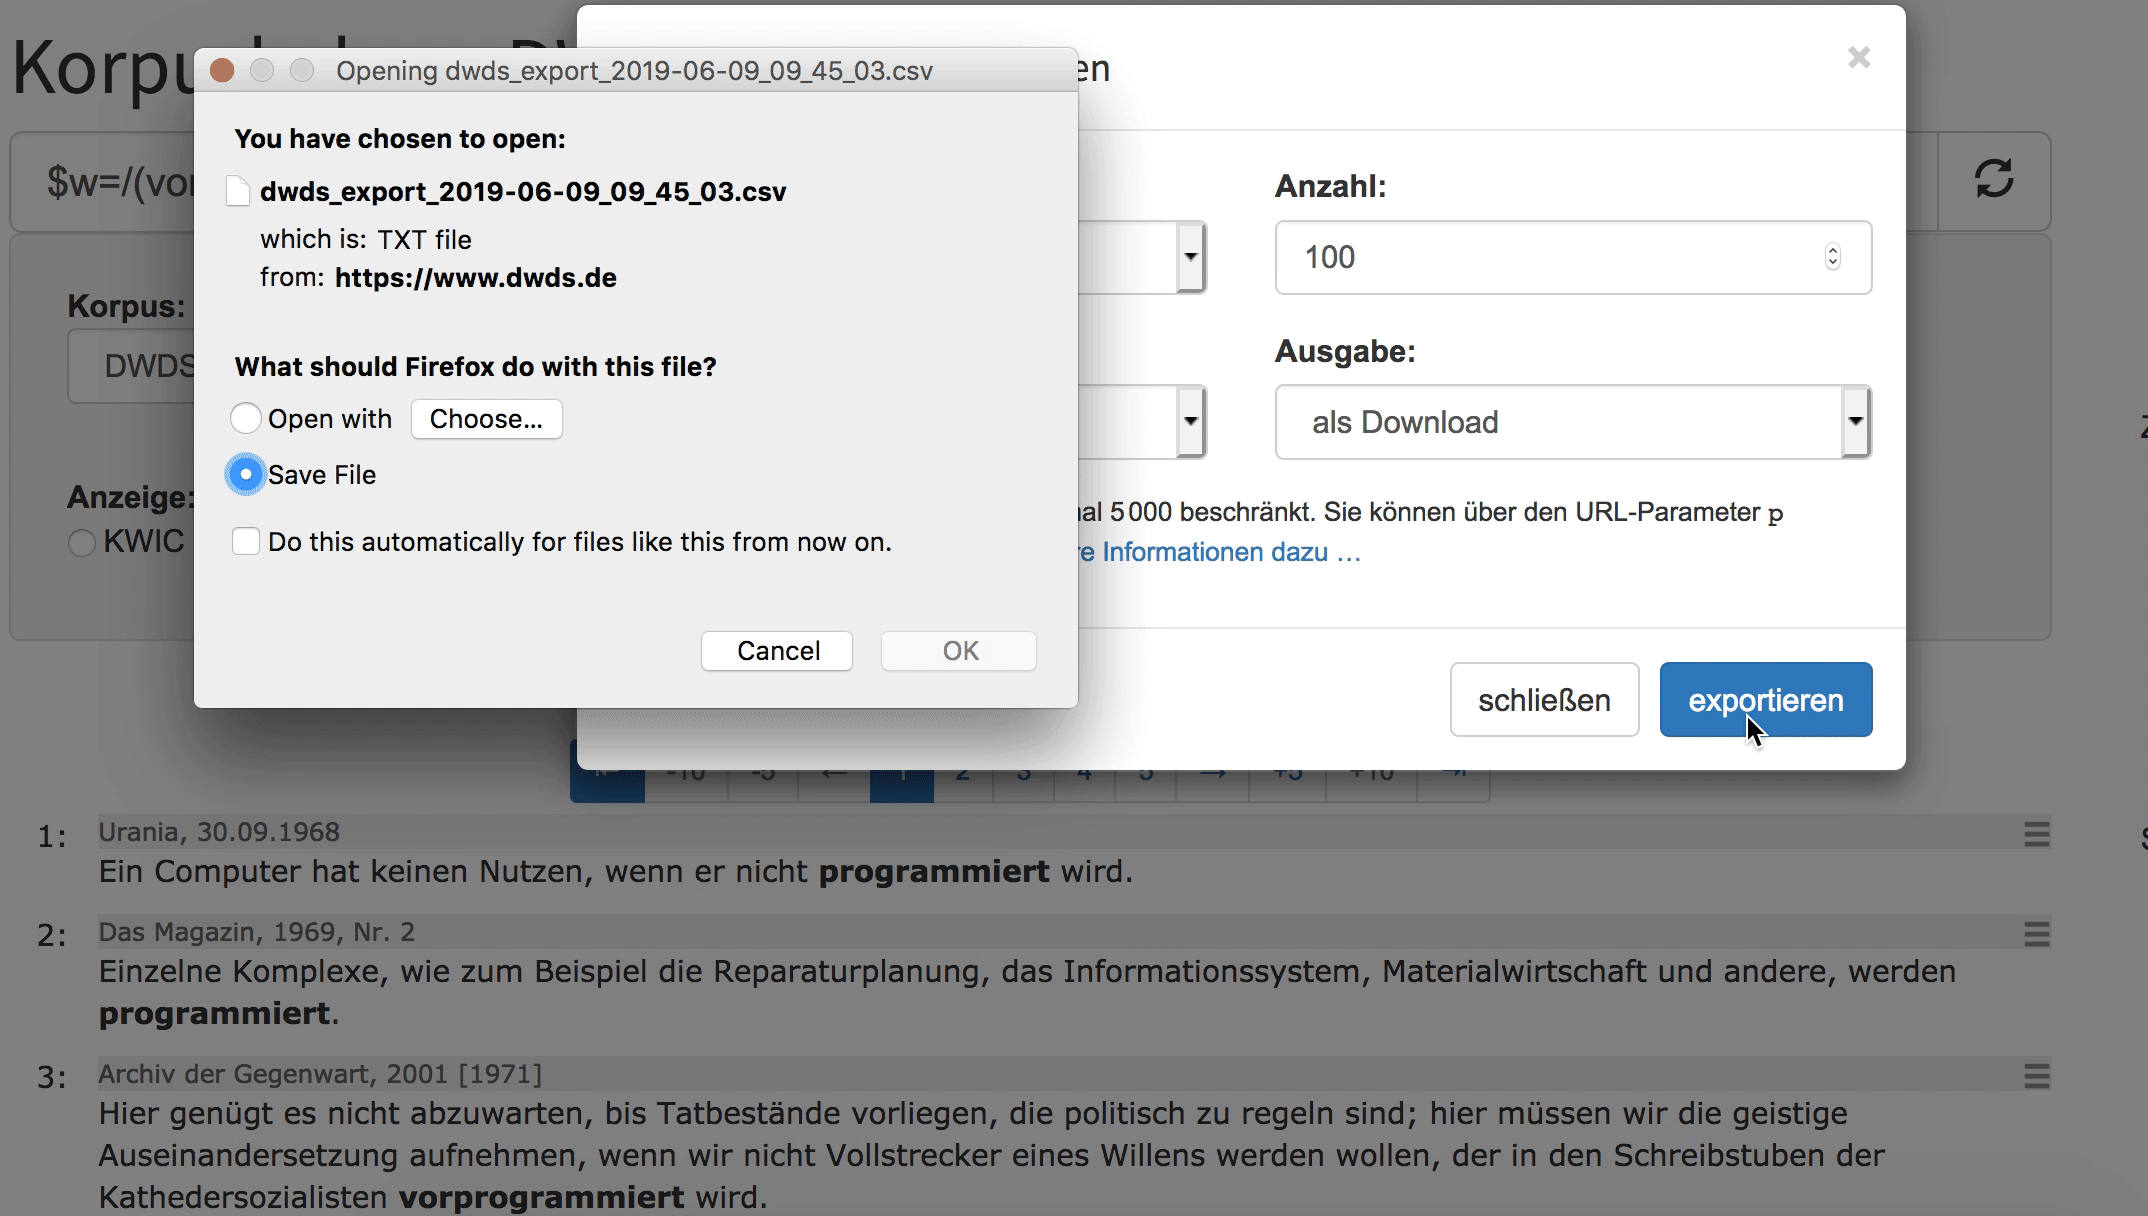
\includegraphics[width=5.37in]{fig/dwdsdownload} \caption{Export aus dem DWDS}\label{fig:dwdsexp}
\end{figure}

Eine solche Sammlung von Korpusbelegen, wie wir sie jetzt exportiert
haben, nennt man in der Korpuslinguistik \textbf{Konkordanz}. Der
Formatname ``CSV'' steht für ``Comma-Separated Values''. Das heißt, in
der Datei sind die einzelnen Werte durch Kommata voneinander abgetrennt.
In einem Texteditor sieht das Ganze so aus wie in \ref{fig:dwdseditor}.
Wie Sie sehen, enthält die Datei neben den Korpusbelegen selbst auch
Metadaten zu den einzelnen Belegen, z.B. zu Autor*in, Titel etc.

\begin{figure}
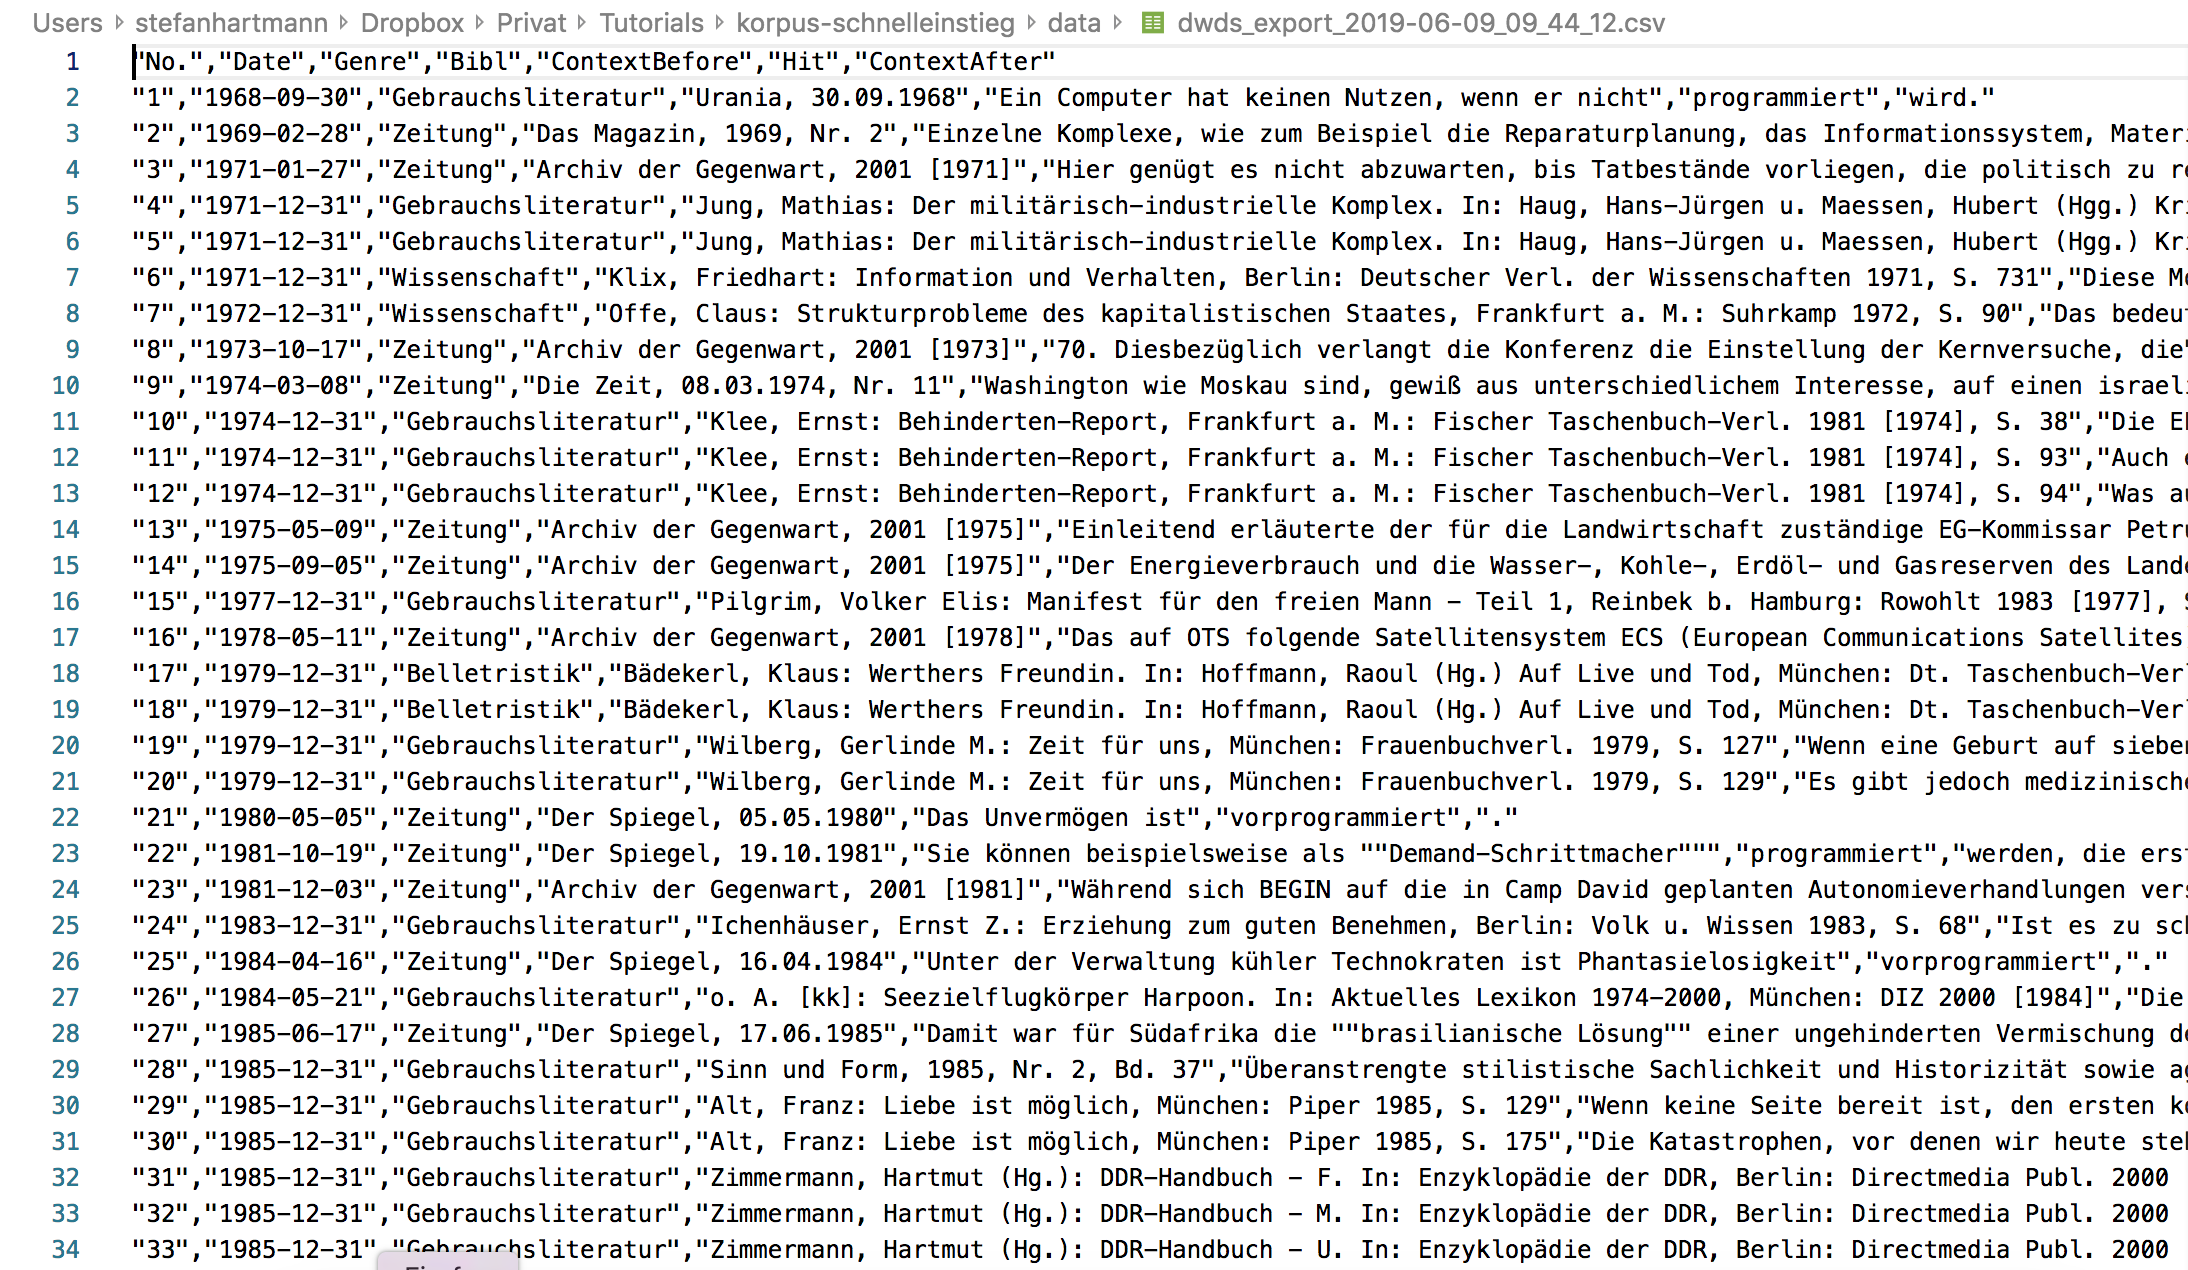
\includegraphics[width=4.86in]{fig/conc_in_editor} \caption{Konkordanz im Texteditor}\label{fig:dwdseditor}
\end{figure}

Damit können wir zunächst noch wenig anfangen: Wir wollen die Konkordanz
in ein Tabellenkalkulationsprogramm einlesen.

\subsubsection{Import in ein
Tabellenkalkulationsprogramm}\label{import-in-ein-tabellenkalkulationsprogramm}

Wenn Sie Microsoft Excel auf Ihrem Rechner installiert haben, sind die
Default-Einstellungen höchstwahrscheinlich so gesetzt, dass CSV-Dateien
in Excel geöffnet werden, wenn Sie darauf doppelklicken. Warum das keine
gute Idee ist, zeigt der folgende Screenshot \ref{fig:excel1} (rote
Hervorhebungen von mir nachträglich hinzugefügt).

\begin{figure}
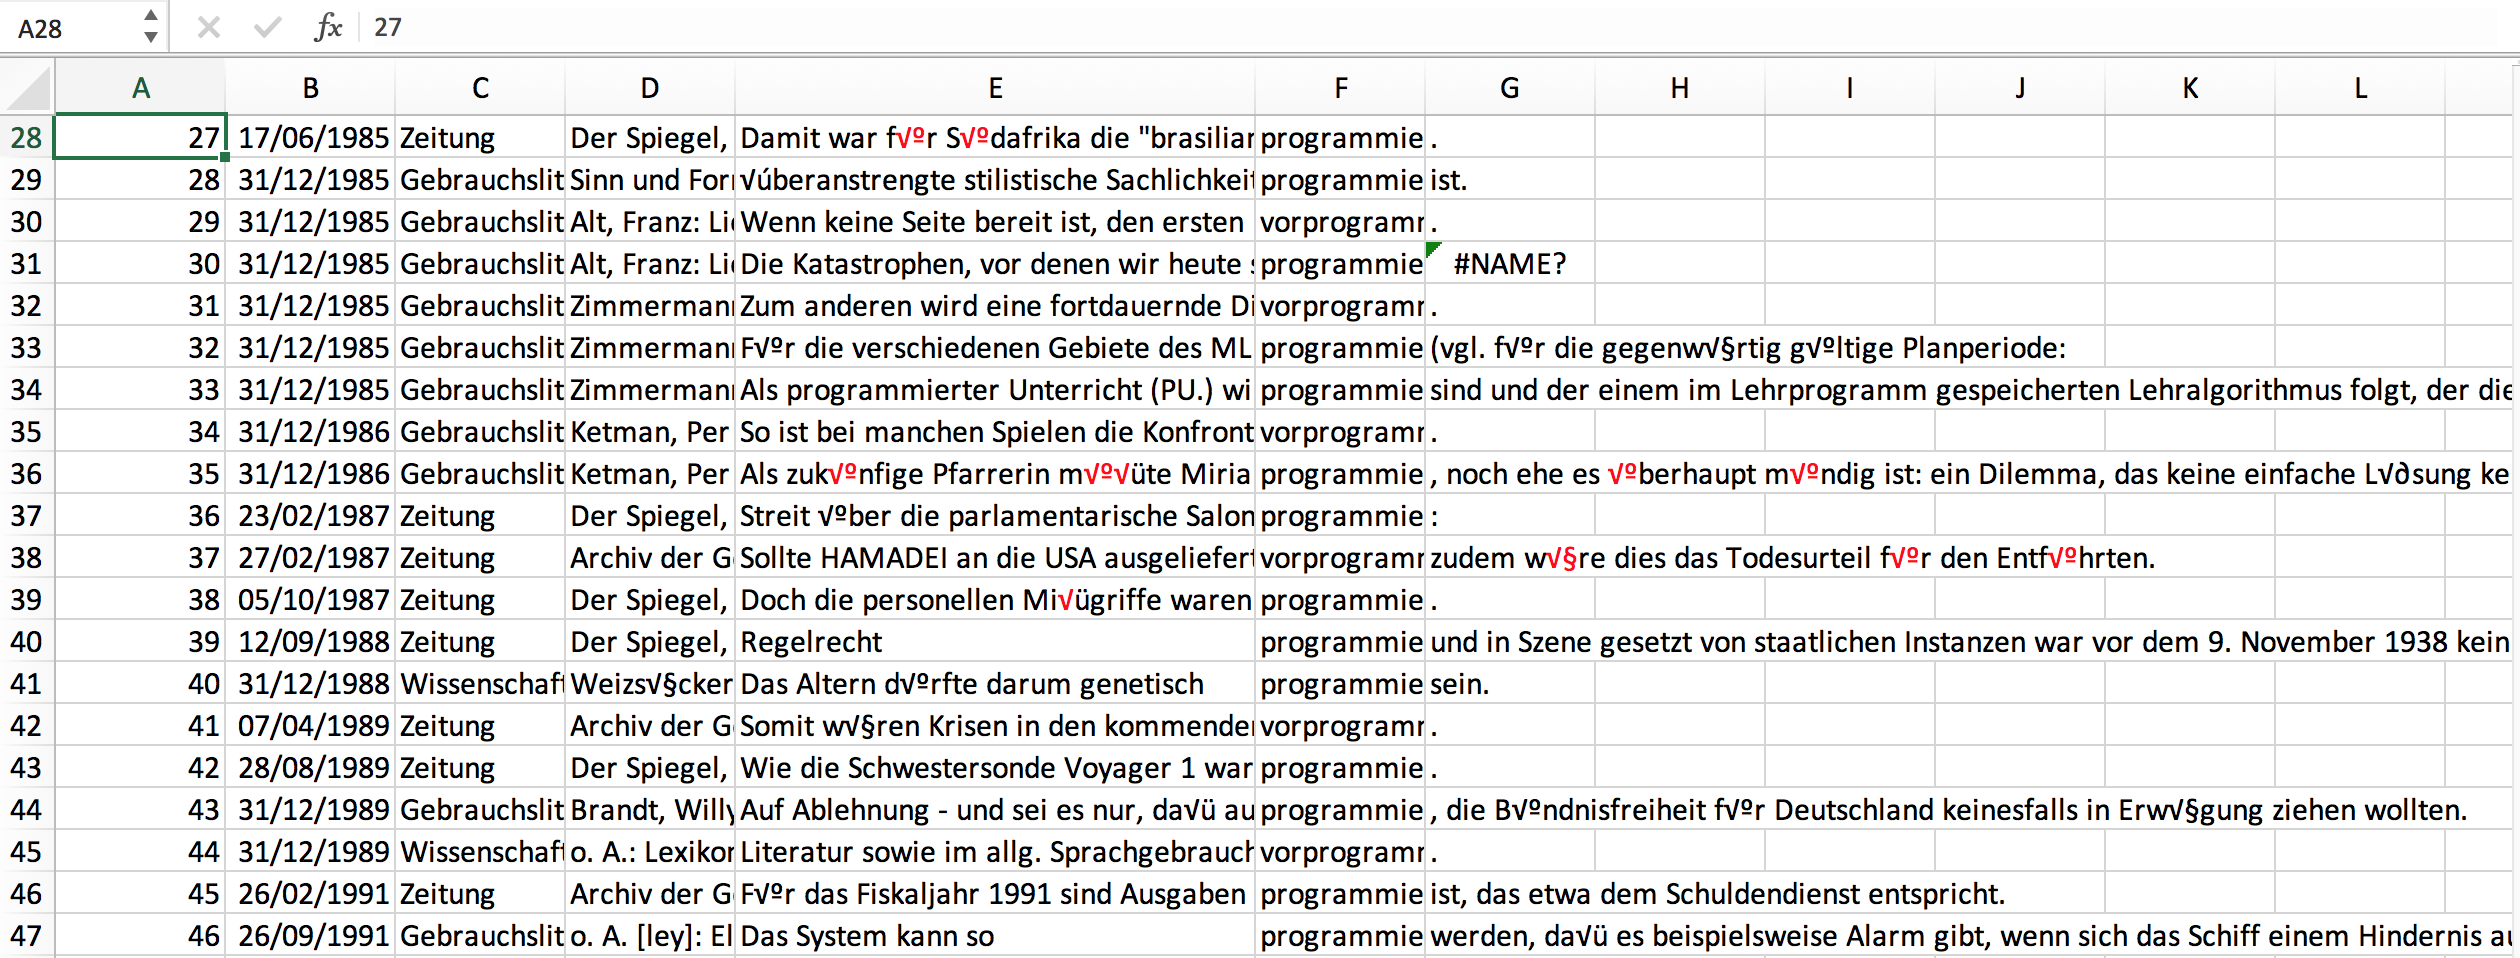
\includegraphics[width=5.04in]{fig/conc_in_excel_bad} \caption{Konkordanz bei direktem Öffnen in Excel}\label{fig:excel1}
\end{figure}

Hier sind einige Sonderzeichen verlorengegangen, weil Excel die
Kodierung der Datei nicht richtig erkannt hat. Es gibt mehrere Wege,
diesem Problem zu begegnen. Ich empfehle hier zwei: Einen für Excel und
einen für die freie Alternative Calc.

\paragraph{Import in Excel}\label{import-in-excel}

\begin{enumerate}
\def\labelenumi{\arabic{enumi}.}
\item
  Öffnen Sie die Datei in einem Texteditor. Für Windows empfehle ich
  Notepad++, für Mac die kostenlose (und für unsere Zwecke völlig
  ausreichende) Version von BBEdit, für Linux gibt es z.B. Notepadqq.
\item
  Markieren Sie mit Strg+A bzw. Cmd+A den gesamten Text.
\item
  Öffnen Sie ein leeres Tabellenblatt in Excel. Die nächsten Schritte, 4
  bis 7, sind in \ref{fig:importexcel} visualisiert.
\item
  In den meisten Fällen sollten Sie nun einfach mit Strg+V bzw. Cmd+V
  die Daten einfügen könnn. In manchen Fällen müssen Sie jedoch, wie im
  Screencast \ref{fig:importexcel}, die Option ``Paste Special''
  verwenden (dt. ``Inhalte einfügen'') und angeben, dass Sie den
  Unicode-Text einfügen möchten.
\item
  Mit Klick auf das kleine Klemmbrett-Symbol gelangen Sie zum
  Textimport-Assistenten. Hier müssen Sie Excel sagen, wie der
  eingefügte Text strukturiert ist. Auf der ersten Seite sagen Sie, dass
  es sich um einen Text handelt, bei dem die einzelnen Spalten durch ein
  Trennzeichen getrennt sind (``Delimited'') - diese Option ist in der
  Regel schon angewählt. Außerdem teilen Sie Excel hier mit, dass der
  eingefügte Text UTF-8-formatiert ist.
\item
  Auf der nächste Seite des Textimport-Assistenten geben Sie an, dass
  Kommata als Spaltentrenner benutzt werden. Bei den Textqualifizierern
  müssen Sie nichts ändern, da hier schon Anführungszeichen ausgewählt
  sind: Wie Sie in \ref{fig:dwdseditor} sehen können, werden
  Anführungszeichen in der CSV-Datei genutzt, um zusammengehörigen Text
  zusammenzuhalten (denn wären sie nicht da, würde Excel jedes Komma im
  Text für einen Spaltentrenner handeln.)
\item
  Dieser letzte Schritt erübrigt sich meistens, kann aber nicht schaden:
  Zuletzt können Sie noch alle Spalten als ``Text'' formatieren. (Die
  Datumsspalte können Sie prinzipiell auch als ``Datum'' formatieren,
  falls Sie ausschließlich in Excel weiterarbeiten, aber tendenziell
  rate ich davon ab - gerade bei einer späteren Konversion in andere
  Dateiformate kann dabei alles mögliche schiefgehen\ldots{})
\end{enumerate}

\begin{figure}
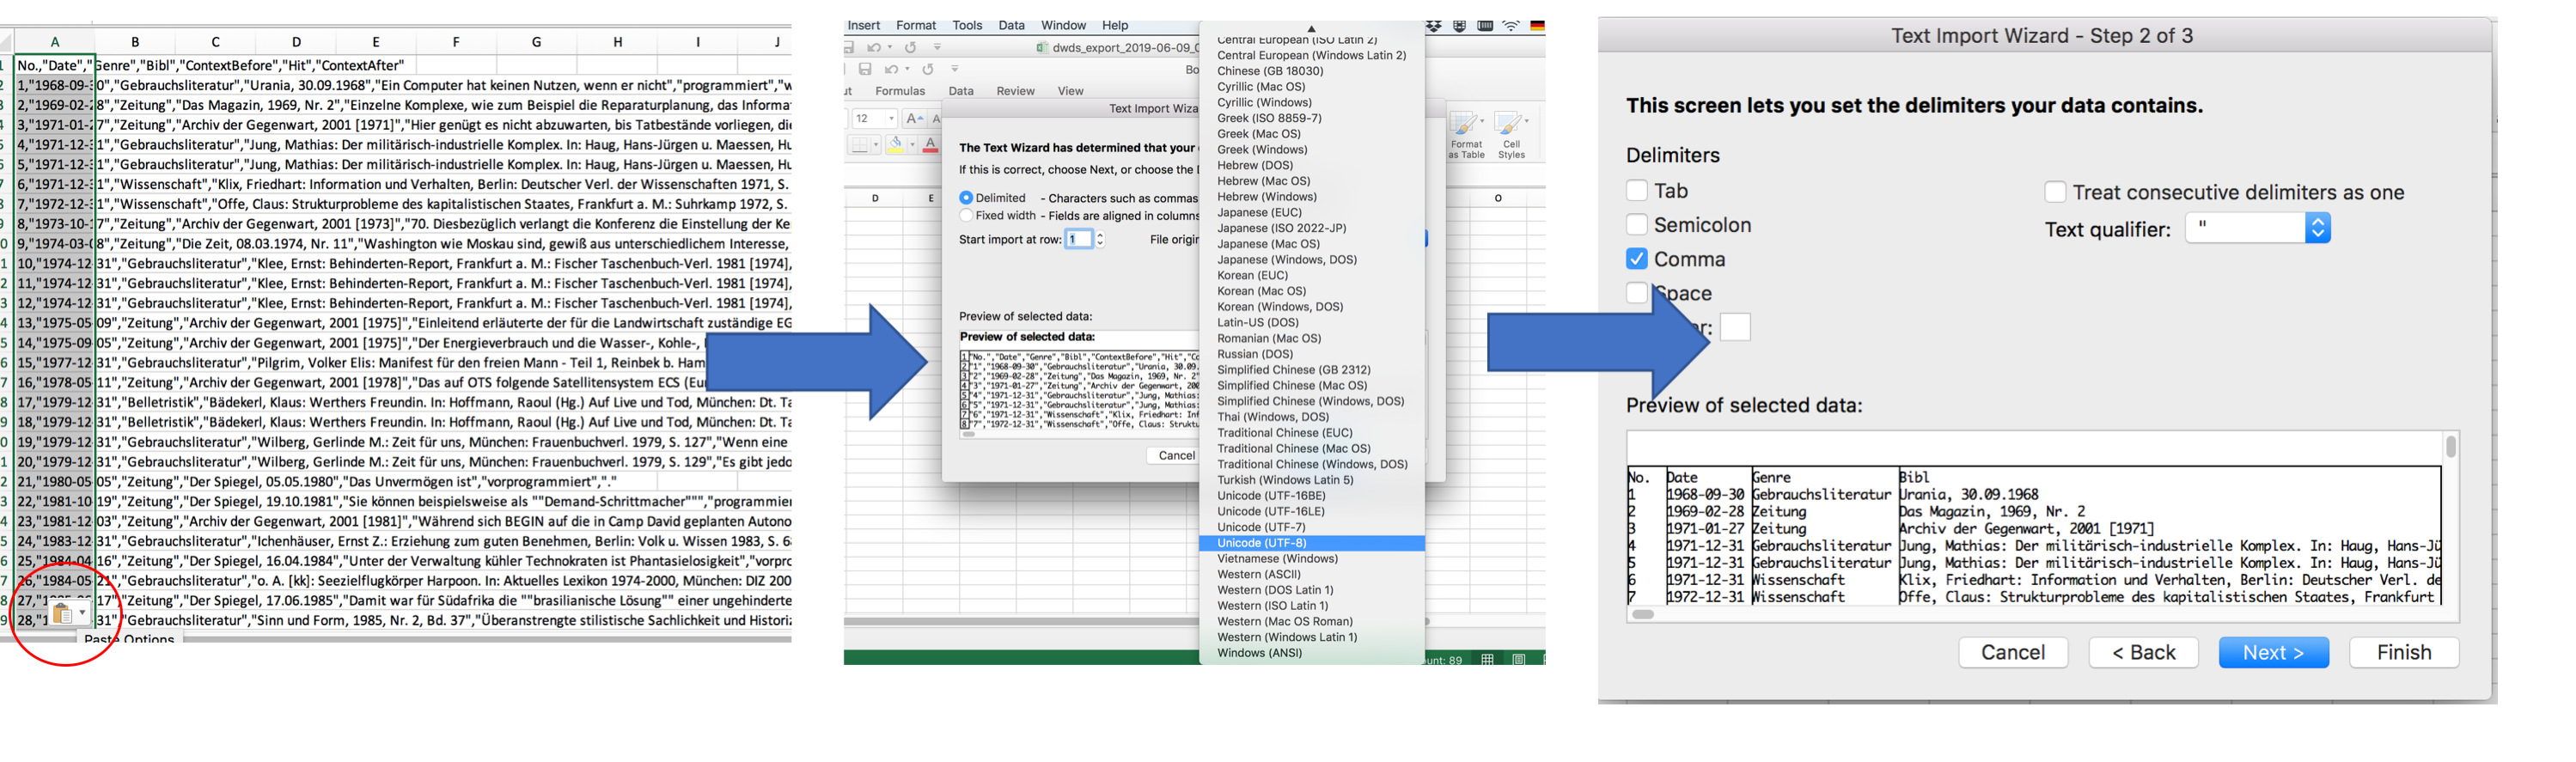
\includegraphics[width=6.66in]{fig/import_in_excel} \caption{Import in Excel}\label{fig:importexcel}
\end{figure}

\paragraph{Import in Calc}\label{import-in-calc}

Öffnet man die Datei im kostenlosen Tabellenkalkulationsprogramm Calc
von LibreOffice (mit Rechtsklick \textgreater{} Öffen mit), so öffnet
sich zunächst automatisch der Textimportassistent. Hier muss man Calc
mitteilen, welches Format die Datei hat. In unserem Fall ist der Text
UTF-8-kodiert, wir haben Kommas als Spaltentrenner und Anführungszeichen
als Textqualifizieren, wie in \ref{fig:calcimport}.

\begin{figure}
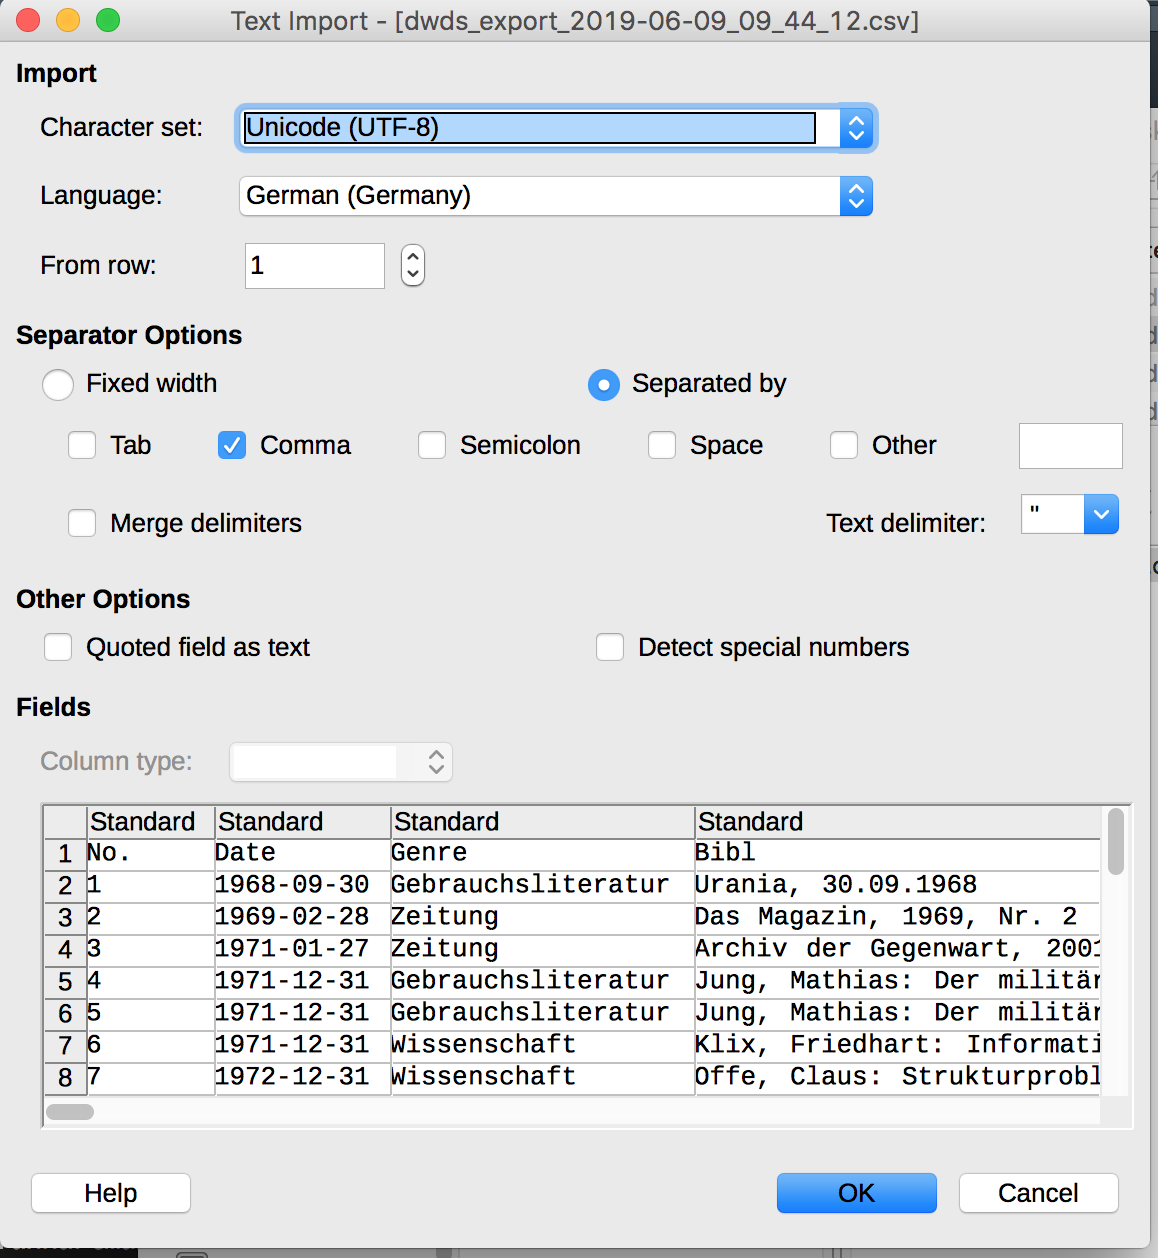
\includegraphics[width=0.5\linewidth,height=0.5\textheight]{fig/calc_import} \caption{Import in Calc}\label{fig:calcimport}
\end{figure}

\section{Von der Konkordanz zur
Analyse}\label{von-der-konkordanz-zur-analyse}

Nun haben wir die Konkordanz erfolgreich in ein
Tabellenkalkulationsprogramm importiert. Hier können wir beliebig viele
weitere Spalten hinzufügen. Das können wir nutzen, um die exportierten
Belege mit \textbf{Annotationen} zu versehen.

\subsection{Annotation}\label{annotation}

Versieht man Daten mit zusätzlichen Informationen, so nennt man diesen
Prozess Annotation. In der Korpuslinguistik stellt die Annotation einen
ganz wesentlichen Schritt dar, der gewissermaßen die Brücke schlägt von
der qualitativ-philologischen Analyse einzelner Belege zur quantitativen
Auswertung.

Wir nutzen im Folgenden die Annotation, um unsere Daten in Kategorien zu
unterteilen, die für unsere Fragestellung sinnvoll sind. Dafür müssen
wir uns zunächst darüber im Klaren sein, was wir von unseren Daten
überhaupt wissen wollen, d.h. wir müssen unsere eingangs genannte
Fragestellung operationalisieren.

Zur Erinnerung: Unsere Fragestellung lautet, ob bei prädikativem
Gebrauch \emph{vorprogrammiert} gegenüber \emph{programmiert} bevorzugt
wird, wenn es sich um einen metaphorischen Kontext handelt.

Konkret bedeutet das, dass wir für jeden Datenpunkt folgende Fragen
beantworten müssen:

\begin{enumerate}
\def\labelenumi{\arabic{enumi}.}
\item
  Handelt es sich um eine prädikative Verwendung? - Schon ein kurzer
  Blick auf die Daten zeigt, dass sich notwendigerweise einige
  \textbf{Fehltreffer} eingeschlichen haben: Häufig finden sich z.B.
  Passivkonstruktionen wie \emph{Es gibt jedoch medizinische Gründe, aus
  denen eine Geburt eingeleitet oder sogar programmiert werden muß}. Uns
  interessieren aber nur Fälle, in denen das Partizip selbst das
  Prädikat bildet, also z.B. \emph{Der Computer ist programmiert} und
  \emph{Die Katastrophe war vorprogrammiert}.
\item
  Handelt es sich um eine metaphorische Verwendung? - Während
  beispielsweise Computer oder Roboter im wörtlichen Sinne programmiert
  werden, bezieht sich der Begriff bei Krisen und Katastrophen darauf,
  dass Voraussetzungen geschaffen wurden, die unausweichlich den
  thematisierten unschönen Ausgang zur Folge haben. Es liegt also ein
  metaphorischer Gebrauch vor, bei der Aspekte der Quelldomäne
  ``Technik'' auf eine abstraktere Zieldomäne übertragen werden.
\end{enumerate}


\end{document}
